\documentclass[journal]{IEEEtran}
\ifCLASSINFOpdf
\else
\fi
\hyphenation{}
\usepackage{amsmath,amssymb,amsthm}
\usepackage{xparse}
\usepackage{latexsym}
\usepackage{amsfonts}
\usepackage{graphicx}
\usepackage{txfonts}
\usepackage{wasysym}
\usepackage{enumitem}
\usepackage{adjustbox}
\usepackage{ragged2e}
\usepackage{tabularx}
\usepackage{changepage}
\usepackage{setspace}
\usepackage{hhline}
\usepackage{multicol}
\usepackage{float}
\usepackage{multirow}
\usepackage{makecell}
\usepackage{fancyhdr}
\usepackage[toc,page]{appendix}
\usepackage[utf8]{inputenc}
\usepackage[T1]{fontenc}
\usepackage{hyperref}
\hypersetup{
    colorlinks=true,
    linkcolor=blue,
    filecolor=magenta,      
    urlcolor=cyan,
}
\usepackage{isomath}
\usepackage{fixmath}
\usepackage{tikz}
\usepackage{textcomp}
\usepackage{epstopdf} %converting to PDF
\usepackage{upgreek}
\usepackage{mathtools}
\usepackage{xfrac}
\usepackage{lipsum}
\usepackage[colorinlistoftodos]{todonotes}
\usepackage[percent]{overpic}
%general:
%Box and color definitions:
%--------------------------
\newenvironment{ColorBoxedminipage}
{\begin{minipage}} {\end{minipage}}
%{\begin{Sbox}\begin{minipage}}
%{\end{minipage}\end{Sbox}\fcolorbox{Blue}{White}{\TheSbox}}

%General definitions:
%-------------------
\newcommand{\etal}{{\em {et al.}}}
\newcommand{\B}[1]{\mathbf{#1}}
\newcommand{\df}{\triangleq}
\newcommand{\norm}[1]{\left\Vert#1\right\Vert}
\newcommand{\abs}[1]{\left\vert#1\right\vert}
\newcommand{\RE}{\operatorname{Re}}
\newcommand{\IM}{\operatorname{Im}}
\newcommand{\sgma}[3]{\sum\limits_{{#1}={#2}}^{#3}}
\newcommand{\Brace}[1]{\left\{{#1}\right\}} %Braces
\newcommand{\Brack}[1]{\left({#1}\right)} %Brackets
\newcommand{\sBrack}[1]{\left[{#1}\right]} %square Brackets

%\newcommand{\ip}[2]{{\langle{#1},{#2}\rangle}} %inner-product
\newcommand{\ipLW}[3]{{\langle{#1},{#2}\rangle}_{{#3}}} %weighted inner-product

\newcommand{\Tr}[1]{Tr\Brack{#1}}
\newcommand{\Mtr}[2] %short notation for 2x1 Matrix.
{\begin{bmatrix}
  #1 \\
  #2
\end{bmatrix}}
\newcommand{\cMtr}[2] %short notation for 2x1 Matrix with curves.
{\left(
\begin{array}{c}
    {#1} \\
    {#2} \\
\end{array}
\right)}
\newcommand{\Mtrs}[2] %short notation for 2x1 Matrix star (adjoint)
{\begin{bmatrix}
  #1 &
  #2
\end{bmatrix}}
\newcommand{\Mtrt}[3] %short notation for 3x1 Matrix.
{\begin{bmatrix}
  #1 \\
  #2 \\
  #3
\end{bmatrix}}

\newcommand{\Cases}[4]{
\left\{
\begin{tabular}{lcl}
    $#1$ & $=$ & $#2$\\
    $#3$     & $=$ & $#4$
\end{tabular}
\right. }

\newcommand{\und}{\underline} %How lazy can I get?
\newcommand{\ovr}{\overline}
\newcommand{\conj}[1]{{#1}^\ast} %Conjugation


\newcommand{\er}[1]{{(\ref{#1})}} %equation reference

\newtheorem{Lemma}{Lemma}{}
\newtheorem{Prop}{Proposition}{}
\newtheorem{theorem}{Theorem}{}


\newenvironment{alg}[5]
{
\begin{figure}[htbp]
\begin{center}
\fbox{
  \begin{ColorBoxedminipage}{13cm}
%    \leftline{\color{Black}\bf {#1}}
    {#4}
   \end{ColorBoxedminipage}
   }
\end{center}
  \bcaptionff{#1}{#2}{}{#3}
  \label{#5}
\end{figure}
}{}

%Just body, caption and label.
\newenvironment{algo}[3]
{
\begin{figure}[htbp]
\begin{center}
\fbox{
  \begin{ColorBoxedminipage}{7.5cm}
%    \leftline{\color{Black}\bf {#1}}
    {#1}
   \end{ColorBoxedminipage}
   }
\end{center}
  \caption{#2}
  \label{#3}
\end{figure}
}{}

\newenvironment{BOX}[1]
{
\begin{center}
\fbox{
  \begin{ColorBoxedminipage}{16cm}
%    \leftline{\color{Black}\bf {#1}}
    {#1}
   \end{ColorBoxedminipage}
   }
\end{center}
}{}

\newcommand\vecnot[1]{\boldsymbol{#1}}
\newcommand\optvecnot[1]{\vecnot{#1}_{opt}}

\usepackage{amsmath}
\DeclareMathOperator*{\argmax}{arg\,max}
\DeclareMathOperator*{\argmin}{arg\,min}
\usepackage{subfig}
\usepackage{stfloats}
%%%%%%%%%%%%%%    aliases    %%%%%%%%%%%%%%
\newcommand{\Brace}[1]{\left\{{#1}\right\}}
\newcommand{\rBrace}[1]{\left({#1}\right)}
\newcommand{\lBrace}[1]{\left|{#1}\right|}
\newcommand{\vBrace}[1]{\left[{#1}\right]}
\newcommand{\cBrace}[1]{\left\{{#1}\right\}}
\newcommand{\dTheta}{\Delta\theta}
\newcommand{\dPhi}{\Delta\phi}
\newcommand{\dOmega}{\Delta\omega}
\newcommand{\dR}{\Delta{R}}
\newcommand{\dTau}{CHANGE_TO_DPHI}
% \newcommand{\D}[2]{\mathcal{D}\rBrace{#1,#2}}
% \newcommand{\Dp}[2]{\mathcal{D}^{#2}\rBrace{#1}}
\newcommand{\D}[2]{\text{D}\rBrace{#1,#2}}
\newcommand{\Dp}[2]{\text{D}^{#2}\rBrace{#1}}

\newcommand{\vd}{\vecnot{d}}
\newcommand{\vx}{\vecnot{x}}
\newcommand{\vAlpha}{\vecnot{\alpha}}
\newcommand{\vBeta}{\vecnot{\beta}}
\newcommand{\vdT}{\vd^{T}}
\newcommand{\vxT}{\vecnot{x}^{T}}
\newcommand{\vAlphaT}{\vAlpha^{T}}
\newcommand{\vBetaT}{\vBeta^{T}}
\newcommand{\vdH}{\vd^{H}}
\newcommand{\vxH}{\vecnot{x}^{H}}
\newcommand{\vAlphaH}{\vAlpha^{H}}
\newcommand{\vBetaH}{\vBeta^{H}}
\newcommand{\vEta}{\vecnot{\eta}}
\newcommand{\vEtaT}{\vEta^{T}}
\newcommand{\vEtaH}{\vEta^{H}}
%\newcommand{\F}[1]{#1^{\mathcal{F}}}
\newcommand{\F}[1]{\MakeUppercase{#1}}
\newcommand{\ePhi}[1]{\exp{\rBrace{#1j\phi}}}
\newcommand{\thetaD}{\theta_{\text{d}}}

\NewDocumentCommand{\evalat}{sO{\big}mm}{%
  \IfBooleanTF{#1}
   {\mleft. #3 \mright|_{#4}}
   {#3#2|_{#4}}%
}

\newcommand{\Steer}[1]{\vd_{#1}} 
\newcommand{\aTd}{\vAlpha^{T}\Steer{}} 
\newcommand{\bTd}{\vBeta^{T}\Steer{}}
\newcommand{\Hr}{\mathcal{H}}
\newcommand{\myTodo}[2]{\ifdefined\showTodo{\todo[#1]{#2}}\else\fi}
\newcommand{\myTodoNew}[2]{\ifdefined\showTodoNew{\todo[#1]{#2}}\else\fi}
% \newcommand{\coefSetName}{\text{CB}}
\newcommand{\coefSetName}{\text{DS}}


%%%%%%%%%%%%%%%%%%%%%%%%%%%%%%%%%%%%%%%%%%%%%%%%%%%%%%
%%%%%%%%%%%%%%      Document flags     %%%%%%%%%%%%%%%
%%%%%%%%%%%%%%%%%%%%%%%%%%%%%%%%%%%%%%%%%%%%%%%%%%%%%%
% \def\showDev{}
% \def\showTodo{}
\def\showTodoNew{}
\def\DEFIncludeAttenuation{}
\def\DEFInclueApplication{}
%%%%%%%%%%%%  Document Code starts here %%%%%%%%%%%%%%
\begin{document}
\title{Source Localization with Feedback Beamforming}
\author{Itay Yehezkel Karo,~\IEEEmembership{}
        Tsvi G. Dvorkind~\IEEEmembership{}
        and 
        Israel Cohen,~\IEEEmembership{Fellow,~IEEE}
\thanks{This work was supported by the Israel Science Foundation (grant no. 576/16), and the ISF-NSFC joint research program (grant No. 2514/17).}
\thanks{Itay Yehezkel Karo and Israel Cohen are with Andrew and Erna Viterby Faculty of Electrical Engineering, Technion -- Israel Institute of Technology, Technion City, Haifa 3200003, Israel (e-mail: itayyeka@gmail.com, icohen@ee.technion.ac.il)}% <-this % stops a space
\thanks{Tsvi G. Dvorkind is with Rafael Advanced Defense Systems, Haifa 31021, Israel (e-mail: dvorkind@rafael.co.il)}% <-this % stops a space
}
\markboth{}%
{}
\maketitle
\begin{abstract}
State-of-the-art array processing methods, ranging from high-order statistics to adaptive configuration, require costly computing efforts in pursuit for spatial performance improvement.
A feedback based approach is introduced in the context of localization, featuring low complexity and high spatial performance in the excess of integrating a transmitter to the array.  
In the proposed scheme, a signal is continuously re-transmitted between the array and the target of interest.
Considering ideal scenarios, the feedback beamformer virtually achieves an infinite aperture, increasing the available spatial information about the target and significantly improves the array's spatial performance.
Using a traditional beamforming performance analysis, the beamwidth, peak to side-lobe ratio, array directivity and white noise sensitivity are evaluated for the feedback based array.
A significant improvement in all aspects is shown, while thoroughly discussing the conditions for enhanced performance.
As a practical and robust implementation of the feedback-based localization concept, an application of low estimation errors sensitivity, 
is presented and analyzed.
\end{abstract}
\begin{IEEEkeywords}
Beamforming, beampattern, cooperative beamforming, source localization, spatial array processing, spatial IIR.
\end{IEEEkeywords}
\section{Introduction}
\IEEEPARstart{T}{he}
\IEEEPARstart{T}{he} 
general field of array processing has been thoroughly studied in many contexts throughout several decades, producing many important applications such as spatial filtering, source localization, signal detection, source separation, manifold learning, feature extraction, and many more.
Spatial sensor arrays enable the extraction of spatial information such as localizing a transmitting source \cite{skolnik2008radar} \myTodo{inline}{\textbf{DONE:}\\cite some radar book}, blindly separating mixtures of impinging signals \cite{Comon1994IndependentConcept} \myTodo{inline}{\textbf{DONE:}\\here you can cite some papers which talk about BSS and ICA signal source separation. Make sure to cite something which is well known, that is, has many citations}, improving signal to noise ratio (SNR) \myTodo{inline}{\textbf{DONE:}\\cite some works/books about MVDR,MPDR processing}\cite{Frost1972AProcessing,verdu1998multiuser} and many more. 
\par Uniform linear array (ULA), a uniformly spaced structure of sensors, has always been a point of interest, due to its simplicity of analysis \cite{VanTrees2002DetectionIV}. 
The array size and the number of its elements ($N$) has significant influence on the obtained array performance, such as SNR improvement, spatial separation capabilities and its number of degrees of freedom (DOF). For example, the influential MUSIC algorithm \cite{Ralph1986MultipleParameter} enables the localization of signals arriving from up to $N-1$ distinctive directions of arrival (DOA), by projecting the the array manifold onto the noise subspace.
\par The inherent limitation on the number of processed or detected sources due to the limited amount of DOF of a given array, inspired different directions of research, aiming to improve the performance of a given array.
\par One approach, involving different array geometries, examined minimum redundancy arrays \cite{Moffet1968Minimum-RedundancyArrays,Pillai1985AEstimation,UnnikrishnaPillai1987StatisticalMatrix}, aiming to reduce the spatial ambiguity. The basic concept was minimization of the inter-element spacing redundancy in order to increase the overall resolution. 
\par Another approach, commonly referenced as ``virtual arrays" \cite{Pal2010NestedFreedom,Chevalier2005OnProcessing,Mendel1999ApplicationsProcessing} deals with the extraction of samples originated in sensors that do not really exist (i.e. relying on higher order statistics and manipulating multiple statistical cross-terms in order to estimate statistical characteristics of signals impinging in missing sensors). 
\par Using a similar approach, the $2q$-MUSIC algorithm \cite{Chevalier2006High-resolutionAlgorithm}, enables the use of $N^{2q}$ ``virtual elements'', by calculating the $q$'th order statistics.
\par This paper is inspired by the well known \cite{VanVeenBeamforming:Filtering} analogy between ULA spatial array processing of narrow-band signals and finite impulse response (FIR) temporal filtering. 
\par In the context of temporal signal processing, it is well known that for a given filter of order $N$, in many cases, the infinite impulse response (IIR) performs better than FIR, considering narrow transition regions and low sidelobes.
\par This naturally arises the question, ``what are the equivalent spatial domain processing methods which will be analogous to temporal IIR filtering?" 
\par A related work \cite{Wen2013ExtendingStructure} has also addressed this question, where in the context of ULA, two approaches were considered.
\par The first one was to estimate the time of arrival (TOA) difference between two consecutive sensors and to synthetically generate the recursive part of the IIR filter, entirely in the time-domain. The second approach suggested to consider overlapping subsets of one large ULA as finite approximation to an infinite array. 
\par Surely, the former approach heavily relies on the accuracy of the delay estimation and the latter approach does not achieve a recursive spatial response. In both cases, there is no true spatial feedback between the array and the source of interest.
\par Other works \cite{Madanayake2008AFilters,Madanayake2008ABeamformer} use the concept of $2D$ spatio-temporal plane wave representation (i.e. a straight line angled according to the DOA in the spatio-temporal plane), to design ultra-wide-band (UWB) filters \cite{L.Bruton1983HighlyPlanes} which both sample spatial snapshots of the signal and recursively process it in temporal domain. \myTodo{inline} {\textbf{REPHRASED}\\please explain (maybe later just to me) how UWB filtering is used}\myTodo{inline}{\textbf{Removed - not important - a way of implementation}\\what is that?}\myTodo{inline}{\textbf{DONE:}\\what are the drawbacks if these last papers?}
Here as well, the recursive part of the filter is obtained entirely in the temporal domain.  
\par In this contribution, we wish to present a sensor array processing approach which achieves the desired spatial domain exclusive IIR-like beampattern, while avoiding any temporal processing of the signal.
\par To this end, we arbitrarily chose to formulate the problem in the context of a localization problem, hence our goal is to estimate the direction and the range of some target of interest. 
\par The novelty, comparing to traditional array processing, is the incorporation of spatial feedback, which we prove to be the spatial domain equivalent of temporal domain IIR filtering.
\par Assuming the target of interest has a mirror-like behaviour (i.e. reflects its impinging signals), the spatial feedback between the array and the target is created by continuously re-transmitting a synthesized version of the impinging signal (and its reflections) to the target.
\par Note that the initial stimulus can be generated by the target or the array itself. In the text to follow, we assume this is the latter. 
\par Moreover, opposed to the passive target case (i.e. a target which merely reflects the impinging signal), one may consider a cooperative target, which receives, enhances and re-transmits the signal back to the array. In this work, we assume the former.
\par The outline of this paper is as follows. We first formulate the classic spatial beamforming setup in Sec.~\ref{sec:setup}. Then, in Sec.~\ref{sec_introduceFeedback}, we propose our novel feedback based architecture, and formulate its spatial response.
Searching for localization performance maximization, Sec.~ \ref{sec_FIM} discuss the information-theory related considerations for the array configuration, utilizing the Fisher Information Matrix (FIM) in the context of the target's range and DOA estimation.
In Sec.~\ref{sec_Performance} we evaluate some key features of the proposed beamforming with feedback. Specifically, we compute the array beamwidth, its peak to sidelobe ratio and the array directivity, showing significant improvement compared to traditional beamforming without spatial feedback. 
In Sec.~\ref{sec_app} we simulate the proposed processing scheme, and emphasis its sensitivity to range errors. We then suggest a strategy which mitigates this sensitivity. Finally, concluding remarks are stated in Sec.~\ref{sec_conclusions}.
\myTodo{inline}{Here you should state the content of the paper. In Sec. \ref{sec:setup} we define our setup. In Sec. ... we analyze the suggested feedback based system. etc...}
\section{Classical Beamforming }\label{sec:setup}
\myTodo{inline}{\textbf{DONE:}\\ why to speak only about ULA? The work is more general and ULA is a special case. Will rephrase this whole section}Consider an $N$-element array with $n$'th sensor at position $p_n,\; n=0,\ldots,N-1$, where we define $p_{0}=0$ to be the reference point for future analysis. Let $p_t$ be the position of a target of interest. We focus on a far field localization problem, aiming for DOA and target range estimation. Without loss of generality, and for simplicity of the exposition, we reduce the discussion to a 2D problem, denoting the DOA by a single angle $\theta_g$. The range $R$ between the array and the target of interest can be computed with respect to some reference sensor, say $p_{0}$, i.e. $R\triangleq\norm{p_{t}-p_{0}}$. 
Inspired by radar based applications, we assume that the signal $x(t)$ is transmitted from the array, reflects back from the target and re-impinges the array, with total time delay of $\tau_{pd}=2R/c$ seconds, where $c$ represents the propagation velocity of the signal in the medium. Opposed to radar applications, we assume that the target of interest is static. 

Let $x_{n,\theta_g}(t)$ be the measured signal at the $n$'th sensor of the array
\begin{equation}
x_{n,\theta_g}(t) = g_{n,\theta_{g}}x\Brack{t-\tau_{pd}-\tau_{n,\theta_{g}}},
\label{eqn:noFeedbackULA_singleSensor_temporal}
\end{equation}
where $g_{n,\theta_{g}}$ represents the gain due to medium attenuation, the influence of target's radar cross section (RCS) and the sensor's gain at DOA $\theta_g$. Here, $\tau_{n,\theta_{g}}$ represents the arrival time difference of the signal between the $n$'th sensor (at $p_n$) and the reference sensors (at $p_{0}$). In the Fourier domain, we can express the array signals in a vector form 
\[
\Steer{\theta_g}x^\mathcal{F}_0(\omega),
\]
where $x^\mathcal{F}_0(\omega)$ is the Fourier transform of the signal on the first element $x_{0,\theta_g}\Brack{t}$ and the $n$'th element of the steering vector is
\begin{equation}
    \label{eq:d}
    \vd_{\theta_g}[n] = g_{n,\theta_{g}}\exp{\rBrace{-j\omega\tau_{n,\theta_g}}},\;n=0,\ldots,N-1 
\end{equation}
is the steering vector. An N element array beamformer which consists of weights $\vBeta$ will then shape the array reception pattern to produce the beamformed signal $\sum_n \beta_n x_{n,\theta}$. The pattern is then given by 
$$ \vBetaT\vd_{\theta_g}x^\mathcal{F}_0(\omega). $$ 
\par For ULA with inter-element spacing $d$, the inter element delay is
$$
\tau_{n,\theta_g}=n\frac{d\cos\Brack{\theta_{g}}}{c}.
$$
Re-writing of the array response in terms of the electric phase
\begin{equation}\label{eq:thetaULA}
\theta=\omega{d\cos\Brack{\theta_{g}}}/{c},
\end{equation}
gives rise to
\[
x^\mathcal{F}_0(\omega)\sum_{n=0}^{N-1}\beta_n
\exp\Brack{-jn\theta}.
\]
Thus, in the ULA case, setting the weights vector $\vBeta$ for obtaining a desired spatial response is mathematically equivalent to FIR filter design~\cite{VanVeenBeamforming:Filtering}.
\par In the standard scheme of processing radar signals, a waveform $x(t)$ is transmitted to, and reflected from the target of interest. Then, the reflected signal is processed by the radar reception array in order to estimate the DOA, range (and Doppler) of the target. On the other-hand, what we propose here is to continuously re-transmit the signal and its echoes back to the platform, such that a spatial feedback loop is created between the array and the target. In the context of ULA, we show this scheme to be equivalent to IIR filter design. The suggested structure is elaborated in Sec.~\ref{sec_introduceFeedback} and analyzed in subsequent sections.

\section{Range Error Sensitivity}
\label{sec_sim}
In this section, we investigate $\HrTPr$ for the general case, where the range misalignment phase term $\dPhi$ may also be non zero. In Fig.~\ref{fig_hDUDTContour}, we plot $\abs{\HrTPr}$ in logarithmic scale, with respect to both steer and range misalignments.
Close inspection of the range error related beampattern behaviour sheds light to some important points.
First, we notice that although setting $r\to1$ (i.e., close to a perfect gain match), sharpens the beampattern's main lobe  (i.e., higher spatial selectivity), it also amplifies the range error ($\dPhi$) related sensitivity as the main lobe's support over the $\dPhi/\pi$ axis shrinks. 
Next, as evident from \eqref{eq_generalH}, the range error related sensitivity is $2\pi$-periodic with respect to $\dPhi$ (see Fig.~\ref{fig_hDUDTContour_mutliPeak}).
To establish our final observation, we first recall that
\[
\phi\triangleq\omega\tau_{pd}=\frac{2\pi R_{\text{rt}}}{\lambda},
\]
where $R_{\text{rt}}=2R$ is the round-trip distance between the array and the target of interest and $\lambda$ is the wavelength. 
Define
\[
\Delta R_{\text{rt}}\omegaB=\frac{\dPhi\lambda}{2\pi} 
\]
to be the range estimation error.
Fig.~\ref{fig_rangError} shows that even minor range errors of $\Delta R_{\text{rt}}\sim0.1\lambda$ significantly distort the beampattern.
\begin{figure}[t!]
    \begin{center}
        \begin{overpic}[width=.9\linewidth, 
        % grid, 
        tics=10,
        % trim={<left> <lower> <right> <upper>}
        trim={0cm 0cm 1.5cm 0cm}
        ]{./Media/spatialIIR_amb_N3_all_r.eps}
            \put (91, 74) {\footnotesize{dB}}
            \put (-2, 22) {$\frac{\dPhi}{\pi}$}
            \put (5, 74) {\footnotesize{$r=0.4$}}
            \put (51, 74) {\footnotesize{$r=0.6$}}
            \put (5, 38) {\footnotesize{$r=0.7$}}
            \put (51, 38) {\footnotesize{$r=0.8$}}
            \put (19, 3) {\footnotesize{$\dTheta/\pi$}}
        \end{overpic}
    \end{center}
    \caption{Evaluation of $10\log_{10}\abs{\Hr_{\dTheta,\dPhi,r}}^2$, considering both steer ($\dTheta$) and range related ($\dPhi$) errors. Centered in each plot, is the 3dB main lobe (white color fill), exemplifying that as the gain mismatch $r$ is set closer to one, we observe an increase of the spatial selectivity (regarding  both $\dTheta$ and $\dPhi$).}
  \label{fig_hDUDTContour}
\end{figure}
\begin{figure}[t!]
    \begin{center}
        \begin{overpic}[width=0.6\linewidth, 
        % grid, 
        tics=10,
        % trim={<left> <lower> <right> <upper>}
        trim={0 0 0 0}
        ]{./Media/spatialIIR_amb_N3r04_multiPeak.eps}
            \put (83, 71) {\tiny{dB}}
            \put (42, -0.5) {\scriptsize{$\dTheta/\pi$}}
            \put (0, 37) {$\frac{\dPhi}{\pi}$}
        \end{overpic}
    \end{center}
    \caption{Evaluation of $10\log_{10}\abs{\Hr_{\dTheta,\dPhi,r=0.4}}^2$ for $-3\pi\leq\dPhi\leq 3\pi$. The response is $2\pi$ periodic.}
  \label{fig_hDUDTContour_mutliPeak}
\end{figure}
\begin{figure}[t!]
    \begin{center}
        \begin{overpic}[width=0.6\linewidth, 
        % grid, 
        tics=10,
        % trim={<left> <lower> <right> <upper>}
        trim={0 0 0 0}
        ]{./Media/rangeError_r06.eps}
            \put (-1, 74) {\footnotesize{$10\log_{10}\abs{\Hr_{\dTheta,\dPhi,r}}^2$}}
            \put (46, -1) {\footnotesize{$\dTheta/\pi$}}
            \put (0, 37) {\footnotesize{dB}}
            \put (92, 40) {\footnotesize{$\Delta R_{\text{rt}}=0.1\lambda$}}
            \put (92, 50) {\footnotesize{$\Delta R_{\text{rt}}=0.3\lambda$}}
            \put (92, 30) {\footnotesize{$\Delta R_{\text{rt}}=0$}}
        \end{overpic}
    \end{center}
    \caption{Evaluation of the array response (where $r=0.4$) for several values of range error $\Delta R_{\text{rt}}$ . Even minor range errors significantly distort the beampattern.}
  \label{fig_rangError}
\end{figure}
\par At first glance, this sensitivity to range errors renders the system being too sensitive for any practical use.
This leads us to seek robust implementations, as elaborated in Sec.~\ref{sec_app}. 

\section{Mitigating Range Error Sensitivity}
\label{sec_app}
As demonstrated in the previous section, the beampattern \eqref{eq_generalH} is very sensitive to range errors, manifested by the phase term $\dPhi=2\pi \Delta R_{rt}/\lambda $. We now propose an architecture which obtains the desired beampattern $\Hr_{\dTheta,\dPhi=0,r}$ even when in practice, the true range to the target is unknown (i.e. $\Delta R_{rt}$ is large). Moreover, we intend to show that the suggested architecture operates at moderately low signal to noise ratio (SNR).

\subsection*{Motivation}
Bearing in mind that the system's phase alignment sensitivity resides in \eqref{eq_generalH} via the  term $\exp\Brack{j\dPhi}=\exp\Brack{j\omega\Delta\tau_{pd}}$, and that the round-trip delay (i.e. $\tau_{pd}$) cannot be controlled, one may suggest to use lower frequencies. Unfortunately, in most cases, this is irrelevant, being physically unfeasible to transmit at very low frequency. Another approach is to simultaneously use several frequencies in order to resolve the range error sensitivity. In the following, we show a possible algorithm which achieves this goal by transmitting with two frequencies $\omega_1$ and $\omega_2$.

\subsection*{Suggested processing scheme}
We use two independently configured instances of the feedback beamformer of Fig.~\ref{fig:Proposed_spatialIIR_ARCH}, such that each instance treats only a specific frequency. This is demonstrated in Fig.~\ref{fig_app}. Assume $x_{i}(t) = e^{j\omega_{i}t}, \omega_{i} = 2\pi{f_{i}}$ with $i=1,2$ are two independent, narrow band, stimuli signals.
\begin{figure}[t!]
    \begin{center}
        \begin{overpic}[width=0.95\linewidth, 
        % grid, 
        tics=10,trim={0 0 0 0}]{./Media/SpatialIIR_APP.png}
            \put (12.5, 64){$\text{FB}_{\vAlpha_{1},\vBeta_{1}}$}
            \put (61, 64){$\text{FB}_{\vAlpha_{2},\vBeta_{2}}$}
            \put (4.5, 59){$y_{1}\rBrace{t}$}
            \put (54, 59){$y_{2}\rBrace{t}$}
            \put (12.9, 41.5){$\text{BPF}_{\omega_{1}}$}
            \put (61.65, 41.5){$\text{BPF}_{\omega_{2}}$}
            \put (6, 51.5){+}
            \put (55, 51.5){+}
            \put (16, 51.5){\footnotesize{$n_{1}\rBrace{t}$}}
            \put (64.75, 51.5){\footnotesize{$n_{2}\rBrace{t}$}}
            \put (24.5, 59){\footnotesize{$\text{Tx}_{1}\rBrace{t}$}}
            \put (73.5, 59){\footnotesize{$\text{Tx}_{2}\rBrace{t}$}}
            \put (36.25, 64){\scriptsize{$x_{1}\rBrace{t}$}}
            \put (43, 64){\scriptsize{$x_{2}\rBrace{t}$}}
            \put (18.25, 13){\footnotesize{Harmonic mean}}
            \put (32, 2){$y\rBrace{t}$}
            \put (54.75, 24){$\Sigma$}
            \put (21.75, 25){\footnotesize{$\mathcal{F}_{\omega_{1}}$}}
            \put (30.75, 25){\footnotesize{$\mathcal{F}_{\omega_{2}}$}}
        \end{overpic}
    \end{center}
    \caption{The suggested dual-frequency beamformer. We use two independent FB blocks (as in Fig.~\ref{fig:Proposed_spatialIIR_ARCH}) and 4 band-pass-filters (BPF) to generate both the transmitted feedback signal ($\text{Tx}_{i}$) and the beamformers' outputs $y_{i}$. $x_{i}$ are the stimuli signals of the FB blocks, while $n_{i}$ are additive noise instances. The blocks marked by $\mathcal{F}_{\omega_{i}}$ compute the Fourier coefficients in $\omega_{i}$ and their outputs feed the harmonic mean calculator which generates the DF beamformer's output.}
    \label{fig_app}
\end{figure}
Note that we do not increase the number of array elements, but merely double the beamformer processing part. The output of each beamformer $y_i(t)$, as well as the re-transmitted feedback signal $\text{Tx}_i(t)$ are filtered by a band pass filter (BPF) around each stimulus frequency. For each beamformer \eqref{eqn:GeneralFeedbackTransferFunction} the output is
\[
y_{i}(t)=H_{\vAlpha_{i},\vBeta_{i}}\rBrace{\omega_{i}}\exp{\rBrace{j\omega_{i}t}}\ \ {i\in\cBrace{1,2}},
\]
where $\vAlpha_{i},\vBeta_{i}$ are the coefficients of the $i$'th beamformer. 
\par We define $H_{\text{DF}}$ to be the \textit{dual frequency} beamformer, which is computed as the harmonic mean of $H_{\vAlpha_{i},\vBeta_{i}}(\omega_i)$ 
\begin{equation*}
    H_{\text{DF}} = \rBrace{H^{-1}_{\vAlpha_{1},\vBeta_{1}}\rBrace{\omega_{1}}+H^{-1}_{\vAlpha_{2},\vBeta_{2}}\rBrace{\omega_{2}}}^{-1}.
\end{equation*}
In practice, $H_{\text{DF}}$ can be estimated by evaluating $y_1(t)$ and $y_2(t)$ in the frequency domain, as also illustrated in Fig.~\ref{fig_app}.

By straight forward derivations, one may deduce that $\lBrace{H_{\text{DF}}}^{-1}$ is
% \begin{equation*}
%     \resizebox{1\linewidth}{!}{
%         \begin{split}
%             \lBrace{H_{\text{DF}}} =
%             \lBrace{
%             \frac
%             {
%             \vBetaT_{1}\vd_{1}\vBetaT_{2}\vd_{2}
%             }{
%             \vBetaT_{2}\vd_{2}\exp{\rBrace{-j\rBrace{\phi_{1}-\phi_{2}}}}+\vBetaT_{1}\vd_{1}
%             -\rBrace{\vBetaT_{1}\vd_{1}\vAlphaT_{2}\vd_{2}+\vBetaT_{2}\vd_{2}\vAlphaT_{1}\vd_{1}}\exp{\rBrace{-j\phi_{2}}}
%             }
%             }.
%         \end{split}
%     }
% \end{equation*}
\begin{equation*}
    \resizebox{1\linewidth}{!}{
        \begin{split}
            \lBrace{
            \frac
            {
            \vBetaT_{2}\vd_{2}\exp{\rBrace{j\rBrace{\phi_{1}-\phi_{2}}}}+\vBetaT_{1}\vd_{1}
            }{
            \vBetaT_{1}\vd_{1}\vBetaT_{2}\vd_{2}
            }
            -
            \frac
            {
            \rBrace{\vBetaT_{1}\vd_{1}\vAlphaT_{2}\vd_{2}+\vBetaT_{2}\vd_{2}\vAlphaT_{1}\vd_{1}}\exp{\rBrace{-j\phi_{2}}}
            }{
            \vBetaT_{1}\vd_{1}\vBetaT_{2}\vd_{2}
            }
            }.
        \end{split}
    }
\end{equation*}
Note that in the special case  where we choose $\vAlpha_{1}=\vBeta_{1}, \vAlpha_{2}=-\vBeta_2{}$, the resultant beampattern is simplified to
\begin{equation}
    \label{eqn_twoFreqApproach_h}
    \abs{H_{\text{DF}}} = \lBrace{\frac{\vBetaT_{1}\vd_{1}}{1+\frac{\vBetaT_{1}\vd_{1}}{\vBetaT_{2}\vd_{2}}\exp{\rBrace{-j\rBrace{\phi_{1}-\phi_{2}}}}}}.
\end{equation}
\par In the general case, the gain of each element is frequency dependant, such that the steering vector $\vd$ of \eqref{eq:d}
can be written as 
\begin{equation*}
    \vd_{\theta_g}[n] = g_{n,\theta_{g}}(\omega)\exp{\rBrace{-j\omega\tau_{n,\theta_g}}},\;n=0,\ldots,N-1.
\end{equation*}
To simplify the exposition, assume that the gain of all the elements is the same, such that $g_{\theta_{g}}(\omega)$ is not a function of the element index $n$. Suppressing also the dependence on the DOA $\theta_g$ (which is the same at both frequencies), the  steering vector at the $i$'th frequency is of the form
\begin{equation}\label{eq:new_d}
\vd_{i}^T=g(\omega_i)\sBrack{\exp{\rBrace{-j\omega_i\tau_{0}}},...,\exp{\rBrace{-j\omega_i\tau_{N-1}}}}.
\end{equation}
Note that the element-wise delay $\tau_n$ is arbitrary, hence we no longer restrict the discussion to linear arrays or any specific array manifold. Also, as $\tau_n$ represents the inter-element delay, we use $\tau_0=0$. 

We further simplify the second beamformer weights to 

% The gain mismatch at each frequency is now
% \[
% r_i= g(\omega_i)/\hat{g}(\omega_i)
% \]
% and we define 
% \begin{equation}
%     \label{eqn_kappa_def}
%     \kappa\triangleq{}r_{1}/r_{2}
% \end{equation}
% to be the gain mismatch ratio, at the two frequencies.

% \par Following \eqref{eq:new_d},
% $$
% \vd_{2}\vBrace{n} =  \rBrace{g(\omega_2)/g(\omega_1)}\vd_{1}\vBrace{n}\exp\rBrace{{-j\rBrace{\phi_{2}-\phi_{1}}}},
% $$
% where $\vd_{i}$ is the steering vector of the impinging signal in $\omega_{i}$.

\begin{equation}\label{eq_simpleBeta}
    \vAlpha_{2}=-\vBeta_{2}=\vBrace{\hat{g}^{-1}(\omega_2),0,\hdots,0}.
\end{equation}
Using \eqref{eq_simpleBeta} within  \eqref{eqn_twoFreqApproach_h} gives rise to 
\begin{equation}
    H_{\text{DF}} = \lBrace{\frac{\vBetaT_{1}\vd_{1}}{1+
    \rBrace{\vBetaT_{1}\vd_{1}/r_{2}}\exp\rBrace{-j\rBrace{\phi_{1}-\phi_{2}}}
    }},
    \label{eq_H_DF_general}
\end{equation}
where $r_i=g(\omega_i)/\hat{g}(\omega_i)$ is the gain mismatch at $\omega_i$. \par Notice that  $H_{\text{DF}}$ is similar to the single frequency (SF) beampattern \eqref{eqn:GeneralFeedbackTransferFunction}, where now the range related phase $\phi$ is replaced by $\phi_{1}-\phi_{2}=(\omega_1-\omega_2)\tau_{pd}$. Hence, by using sufficiently close frequencies, range mismatches can be controlled and significantly mitigated.
\par For example, consider a radio frequency carrier of $10\text{GHz}$ and typical range error of $\Delta{}R_{rt}=10_m$, which is $333\frac{1}{3}\lambda$ (assuming light speed of $c=3\cdot 10^{8}_{m/s}$). The single frequency beampattern distortion, being periodic in $\lambda$, will be distorted as for $\Delta{}R_{rt}=\lambda/3$, which is similar to the $0.3\lambda$ error plot presented in Fig.~\ref{fig_rangError}. 
\par Assume that we aim at maximal phase error of $\Delta \phi=0.01\pi_{rad}$. For the dual frequency beamformer, this can be achieved by requiring
\begin{equation}\label{eq_DF_phErr}
\abs{(\omega_1-\omega_2)\frac{\Delta{}R_{rt}}{c}}<0.01\pi,
\end{equation}
or equivalently, for maximal range error of $10_m$, one needs to use two frequencies with separation of
\[
\abs{f_1-f_2}<0.005 c/\Delta{}R_{rt}=150_{KHz}. 
\]

\subsection*{Dual frequency $\coefSetName$ simulation}
We now simulate \eqref{eq_H_DF_general} for the $\coefSetName$ approach assuming ULA. Using coefficients $\vBeta_{1}$ which will coherently sum the wave-front, while minimizing the magnitude of the denominator, we use
\begin{equation*}
    \vBeta_{1}=-\hat{\vd}^{\ast}\exp\rBrace{j\rBrace{\hat{\phi}_{1}-\hat{\phi}_{2}}}/\norm{\hat{\vd}}^2
\end{equation*}
where $\hat{\vd}$ is the estimated steering vector, as in \eqref{eq:d_hat}. With this choice, and similarly to \eqref{eq:SF_CB}, \eqref{eq_H_DF_general} becomes
\begin{equation}
    \label{eqn_H_DF_CB}
    \resizebox{.89\linewidth}{!}{
        \begin{split}
            H_{\text{DF,CB}} =
            \lBrace{\frac{r_{1}\D{\dTheta/2}{N}}{1-
            \kappa\D{\dTheta/2}{N}\exp\rBrace{-j\rBrace{\dPhi_{2}-\dPhi_{1}+(N-1)\dTheta/2}}}
            },
        \end{split}
    }
\end{equation}
where $\kappa\triangleq{}r_{1}/r_{2}$ is the gain mismatch ratio. Note that if the array elements have similar gain at $\omega_1$ and $\omega_2$ we also mitigate the gain mismatch, as $\kappa$ will be close to one.
In Fig.~\ref{fig_dualfreq_rangeErrorHighSnr}, we simulate the beampattern (normalized to $0$dB peak gain) for the single and dual frequency case. We also plot (in blue circles) the perfectly aligned pattern, which is obtained when there are no range errors. As can be seen, the resultant beampattern of the dual frequency beamformer is very close to the, ideal, range-error free case. 

In Fig.~\ref{fig_dualfreq_perfectAlignLowSnr}
we repeat the case of fractional range error of $\Delta{}R_{rt}=0.3\lambda$, while adding white Gaussian noise to the output of each feedback beamformer.
As can be seen, the suggested approach operates reasonably well also in the noisy scenario. 
% \begin{figure}[t!]
%     \begin{center}
%         \begin{overpic}[width=.9\linewidth, 
%         % grid, 
%         tics=10,trim=0 0 0 0]{./Media/fig_dualfreq_perfectAlignHighSnr.png}
%             \put (38, 43.85){\scriptsize{theory BP}}
%             \put (38, 40.85){\scriptsize{SF}}
%             \put (38, 38){\scriptsize{DF}}
%             \put (-5, 25){\footnotesize{dB}}
%             \put (-6, 48) {\footnotesize{$10\log_{10}\abs{\Hr_{\dTheta,\dPhi=0,r=0.6}}^2$}}
%             \put (21, -3){\footnotesize{$\dTheta/\pi$}}
%         \end{overpic}
%     \end{center}
%     \caption{We simulate 3 sensor array with $r=\kappa=0.6$ under the perfect alignment scenario, and show that both the SF and DF beampatterns accurately follow the theoretical result. We also demonstrate the beam steering ability, such that the left plot is for $\theta_{g,s}=\pi/2$ and the right is for $\theta_{g,s}=3\pi/4$.}
%     \label{fig_dualfreq_perfectAlignHighSnr}
% \end{figure}
\begin{figure}[t!]
    \begin{center}
        \begin{overpic}[width=.7\linewidth, 
        % grid, 
        tics=10,trim=0 0 0 0]{./Media/fig_dualfreq_rangeErrorHighSnr.eps}
            \put (47.5, 43){\scriptsize{Ideal}}
            \put (47.5, 37.5){\scriptsize{SF}}
            \put (47.5, 32){\scriptsize{DF}}
            \put (2, 37.5){\footnotesize{dB}}
            \put (47,0){\footnotesize{$\dTheta/\pi$}}
            \put (92,58){\footnotesize{$\Delta{}R_{rt}=0.3\lambda$}}
        \end{overpic}
    \end{center}
    \caption{Simulating 3 element ULA with $r_1=0.6^{2},\; r_2=0.6$ (hence $\kappa=0.6$) for infinite SNR. The (fractional) range error is $\Delta{}R_{rt}=0.3\lambda$.
    Comparing the ideal response which would be obtained for $\Delta{}R_{rt}=0$ (blue dots), with the single frequency (SF) beamformer (red squares) and the  dual-frequency (DF) solution (green diamonds). 
    For the latter, the frequency separation was configured to obtain range errors as in \eqref{eq_DF_phErr}, i.e. $f_1=10_{GHz},\;f_2=f_1+150_{KHz}$ to mitigate range errors up till $\Delta{}R_{rt}=10_m=333\frac{1}{3}\lambda$. 
    }
    \label{fig_dualfreq_rangeErrorHighSnr}
\end{figure}
\begin{figure}[t!]
    \begin{center}
        \begin{overpic}[width=0.9\linewidth, 
        % grid, 
        tics=10,
        % trim={<left> <lower> <right> <upper>}
        trim={1.75cm 0 1.75cm 0}
        ]{./Media/fig_dualfreq_rangeErrorLowSnr.eps}
            \put (42,17.5){\scriptsize{Ideal}}
            \put (42, 14.5){\scriptsize{SF}}
            \put (42, 11.75){\scriptsize{DF}}
            \put (-1, 26.5){\footnotesize{dB}}
            \put (22, 0){\footnotesize{$\dTheta/\pi$}}
            \put (20,17){\scriptsize{$\text{SNR}=6_{dB}$}}
            \put (72,17){\scriptsize{$\text{SNR}=0_{dB}$}}
        \end{overpic}
    \end{center}
    \caption{Directional response of the 3 element ULA, as in Fig.~\ref{fig_dualfreq_rangeErrorHighSnr}, simulated for the noisy scenario. The additive noises $n_1(t)$ and $n_2(t)$ (see Fig.~\ref{fig_app}), are set to obtain SNR of $6_{dB}$ (left plot) and $0_{dB}$ (right plot). The dual-frequency beamformer (green diamonds) achieves close-to-ideal beampattern (blue circles), while the single-frequency approach (red squares) suffers severe distortions.}
    \label{fig_dualfreq_perfectAlignLowSnr}
\end{figure}
\section{Conclusions}
\label{sec_conclusions}
Integrating feedback into standard beamformers proved to achieve the spatial domain equivalent of the temporal IIR filtering.
It seems that a simple generalization of the conventional-beamformer maximizes (locally) the system's spatial information, thus enabling high localization accuracy.
The feedback-based architecture performance evaluation predicts an unlimited improvement in all criteria, when considering perfect knowledge of the target's range and the channel attenuation.
It turns out that a single frequency waveform based feedback-beamformer is impractical, being too sensitive to even mild target range estimation errors.
Fortunately, using a dual-frequency waveform and applying simple frequency domain manipulations to the output and feedback signals, were found to serve as a low frequency (hence low sensitivity) equivalent of the single frequency scheme.
Also, the dual frequency scheme proved to be of low noise sensitivity, featuring high performance even in relatively low signal-to-noise-ratio scenarios.
\par Future study of the feedback beamforming concept may be applied to other array processing applications other than localization.
Furthermore, it is worthwhile to inspect other interesting choices of coefficients rather than the conventional-beamformer generalization, other waveforms and associated processing schemes, to extend the results to dynamic/multiple targets and to consider sensors with general radiation patterns.
Also, one may consider generalizing the suggested architecture to multiple-input-multiple-output systems, enabling a steered/focused (rather than omni-directional) feedback transmission.

\section*{Acknowledgement}
The authors thank the anonymous reviewers for their constructive comments which helped to improve the presentation of this paper.

\appendices
\section{FIM calculation}
\label{apdx_clacFim}
Following \eqref{eq_beamPatternFreqDomain_FIM}, we elaborate the steps leading to \eqref{eqn_FIMelements}. First, we express the parial derivatives of $\F{y}$ with respect to $\vEta$, resulting in
\begin{equation*}
    \resizebox{.9\linewidth}{!}{
        \begin{split}
            \frac{\partial{\F{y}}}{\partial{\theta_{g}}} &= 
            \frac{
            \vBetaT{}A\vd\ePhi{-}\rBrace{1-\aTd\ePhi{-}}+\bTd\vAlphaT{}A\vd\ePhi{-2}
            }{
            \rBrace{1-\aTd\ePhi{-}}^{2}
            }
            \\&=
            \frac{
            \vBetaT{}A\vd\ePhi{-}-\vBetaT{}\rBrace{A\vd\vdT-\vd\vdT{}A}\vAlpha\ePhi{-2}
            }{
            \rBrace{1-\aTd\ePhi{-}}^{2}
            }
            \\&=
            \frac{
            \vBetaT{}A\vd\ePhi{-}-\vBetaT{}B\vAlpha\ePhi{-2}
            }{
            \rBrace{1-\aTd\ePhi{-}}^{2}
            }
        \end{split}
    }
\end{equation*}
and
\begin{equation*}
    \resizebox{.9\linewidth}{!}{
        \begin{split}
            \frac{\partial{\F{y}}}{\partial{\phi}} &= 
            \frac{
            -j\bTd\ePhi{-}\rBrace{1-\aTd\ePhi{-}}-j\bTd\aTd\ePhi{-2}
            }{
            \rBrace{1-\aTd\ePhi{-}}^{2}
            }
            \\&=
            \frac{
            -j\bTd\ePhi{-}
            }{
            \rBrace{1-\aTd\ePhi{-}}^{2}
            }
        \end{split}
    }
\end{equation*}
such that
\begin{equation*}
    % \resizebox{.9\linewidth}{!}{
        \begin{split}
            J_{\theta_{g}\theta_{g}} &= \Re\cBrace{\frac{1}{2\pi\sigma^{2}}\int_{-\omega_{s}/2}^{\omega_{s}/2}\lBrace{\frac{\partial{\F{y}(\omega)}}{\partial{\theta_{g}}}}^{2}d\omega}
            \\&=
            \frac{1}{2\pi\sigma^{2}}\int_{-\omega_{s}/2}^{\omega_{s}/2}{\frac{
            \lBrace{\vBetaT{}A\vd-\vBetaT{}B\vAlpha\ePhi{-}}^{2}
            }{
            \lBrace{1-\aTd\ePhi{-}}^{4}
            }\lBrace{\F{x}(\omega)}^{2}d\omega},
            \\
            J_{\phi\phi} &= \Re\cBrace{\frac{1}{2\pi\sigma^{2}}\int_{-\omega_{s}/2}^{\omega_{s}/2}\lBrace{\frac{\partial{\F{y}(\omega)}}{\partial{\phi}}}^{2}d\omega}
            \\&=
            \frac{1}{2\pi\sigma^{2}}\int_{-\omega_{s}/2}^{\omega_{s}/2}{\frac{
            \lBrace{\bTd}^{2}
            }{
            \lBrace{1-\aTd\ePhi{-}}^{4}
            }\lBrace{\F{x}(\omega)}^{2}d\omega}
        \end{split}
    % }
\end{equation*}
and the cross terms are
\begin{equation*}
    \resizebox{.9\linewidth}{!}{
        \begin{split}
            &J_{\theta_{g}\phi} = J_{\phi\theta_{g}}^{\ast} = 
            \\&= \Re\cBrace{\frac{1}{2\pi\sigma^{2}}\int_{-\omega_{s}/2}^{\omega_{s}/2}
            \rBrace{\frac{\partial{\F{y}(\omega)}}{\partial{\phi}}}^{\ast}
            \frac{\partial{\F{y}(\omega)}}{\partial{\theta_{g}}}d\omega}
            \\&=
            \Re\cBrace{\frac{1}{2\pi\sigma^{2}}\int_{-\omega_{s}/2}^{\omega_{s}/2}{\frac{
            j\vBetaT{}\rBrace{A\vd-B\vAlpha\ePhi{-}}\vdH\vBeta^{\ast}
            }{
            \lBrace{1-\aTd\ePhi{-}}^{4}
            }\lBrace{\F{x}(\omega)}^{2}d\omega}}.
        \end{split}
    }
\end{equation*}
Analyzing the cross terms, we find that for $\vAlpha,\vBeta\propto\vd^{\ast}$ the $\vBetaT{}B\vAlpha$~term vanishes. Assuming real input and real gain terms $g_n$ within the steering vector, the function
\[
\frac{\lBrace{\F{x}(\omega)}^{2}}{\lBrace{1-\aTd\ePhi{-}}^{4}}
\]
is even in $\omega$, and $j\vBetaT A \vd\vdH\vBeta^\ast \propto j\vBetaT A \vd \norm{\vd}^2$ is odd. Hence the cross terms vanish.

\section{Half power beamwidth}
\label{apdx_HPBW}
We now equate the squared norm of \eqref{eq_Hdphi0} to $0.5$ and compute the value of $N\dTheta/2$ for large $N$. To this end, we denote $\gamma\triangleq\dTheta/2$, giving rise to
\begin{equation*}
    \resizebox{1\linewidth}{!}{
        \begin{split}
            \abs{\Hr_{\dTheta,\dPhi=0,r}\rBrace{\omega}}^{2}&=
             \frac{\rBrace{1-r}^{2}\Dp{\gamma,N}{2}}{\abs{\exp\rBrace{j(N-1)\gamma}-r\D{\gamma}{N}}^{2}}
             \\&
             \overset{N\gg1}{\approx}\frac{\rBrace{1-r}^{2}\Dp{\gamma,N}{2}}{1-2r\cos{\rBrace{N\gamma}}\D{\gamma}{N}+r^{2}\Dp{\gamma,N}{2}}
        \end{split}
    }
\end{equation*}
,which is compared to $1/2$, leading to
\begin{equation*}
    % \resizebox{1\linewidth}{!}{
        \begin{split}
            \rBrace{r^{2}-4r+2}\Dp{\gamma,N}{2}+2r\cos{\rBrace{N\gamma}}\D{\gamma}{N}-1 = 0.
        \end{split}
    % }
\end{equation*}
Since for large $N$, the main lobe width goes to zero, we approximate $\sin(\gamma)$ with $\gamma$. Also defining $x\triangleq{}N\gamma=N\dTheta/2$ we obtain \eqref{eq_HPBW}.

\section{Proof of Theorem \ref{thrm_DF}}
\label{apdx_thrm_DF}
\begin{proof}
    Elaborating \eqref{eqn_HDF_def} gives rise to
    \fi
    \begin{equation*}
        \centering
            \begin{split}
                Z_{\text{DF}}^{-1}
                =&                    \abs{\frac{1-\gI{1}\vAlphaHI{1}\vdI{1}e^{{-j\phiI{1}}}}{\gI{1}\vBetaHI{1}\vdI{1}e^{{-j\phiI{1}}}} + \frac{1-\gI{2}\vAlphaHI{2}\vdI{2}e^{{-j\phiI{2}}}}{\gI{2}\vBetaTI{2}\vdI{2}e^{{-j\phiI{2}}}}}
                \\
                =&
                \resizebox{.9\linewidth}{!}{                    \abs{\frac{\gI{2}\vBetaHI{2}\vdI{2}e^{{-j\phiI{2}}}-\gI{1}\gI{2}\rBrace{\vAlphaHI{1}\vdI{1}\vBetaHI{2}\vdI{2}+\vAlphaHI{2}\vdI{2}\vBetaHI{1}\vdI{1}}e^{-j\rBrace{\phiI{1}+\phiI{2}}}+\gI{1}\vBetaHI{1}\vdI{1}e^{{-j\phiI{1}}}}
                {
                \gI{1}\vBetaHI{1}\vdI{1}\gI{2}\vBetaHI{2}\vdI{2}
                }}
                }
                \\
                =&
                \resizebox{.9\linewidth}{!}{
                \abs{
                \frac
                {                    \gI{2}\vBetaHI{2}\vdI{2}e^{{j\rBrace{\phiI{1}-\phiI{2}}}}+\gI{1}\vBetaHI{1}\vdI{1}
                }{
                \gI{1}\vBetaHI{1}\vdI{1}\gI{2}\vBetaHI{2}\vdI{2}
                }
                -\frac
                {                    \rBrace{\vBetaHI{1}\vdI{1}\vAlphaHI{2}\vdI{2}+\vBetaHI{2}\vdI{2}\vAlphaH_{1}\vdI{1}}e^{{-j\phiI{2}}}
                }{
                \vBetaHI{1}\vdI{1}\vBetaHI{2}\vdI{2}
                }
                }
                }.
            \end{split}
    \end{equation*}
    Note that in the special case of choosing $\vAlphaI{1}~=~\vBetaI{1},\ \vAlphaI{2}~=~-~\vBetaI{2}$, the resultant beampattern simplifies to
    \begin{equation*}
        Z_{\text{DF}} = \lBrace{\frac{\gI{1}\vBetaHI{1}\vdI{1}}{1+\frac{\gI{1}\vBetaHI{1}\vdI{1}}{\gI{2}\vBetaHI{2}\vdI{2}}\exp{\rBrace{-j\rBrace{\phiI{1}-\phiI{2}}}}}}.
    \end{equation*}
    Also setting
    $\vBetaI{2}=\vBrace{-1/\gIHat{2},0,\hdots,0}$
    results in \eqref{eqn_H_DF_general}.
\end{proof}
\ifCLASSOPTIONcaptionsoff
  \newpage
\fi
\bibliographystyle{IEEEtran}
\bibliography{./Modules/LocalBib}% ./Modules/LocalBib}
\begin{IEEEbiography}[{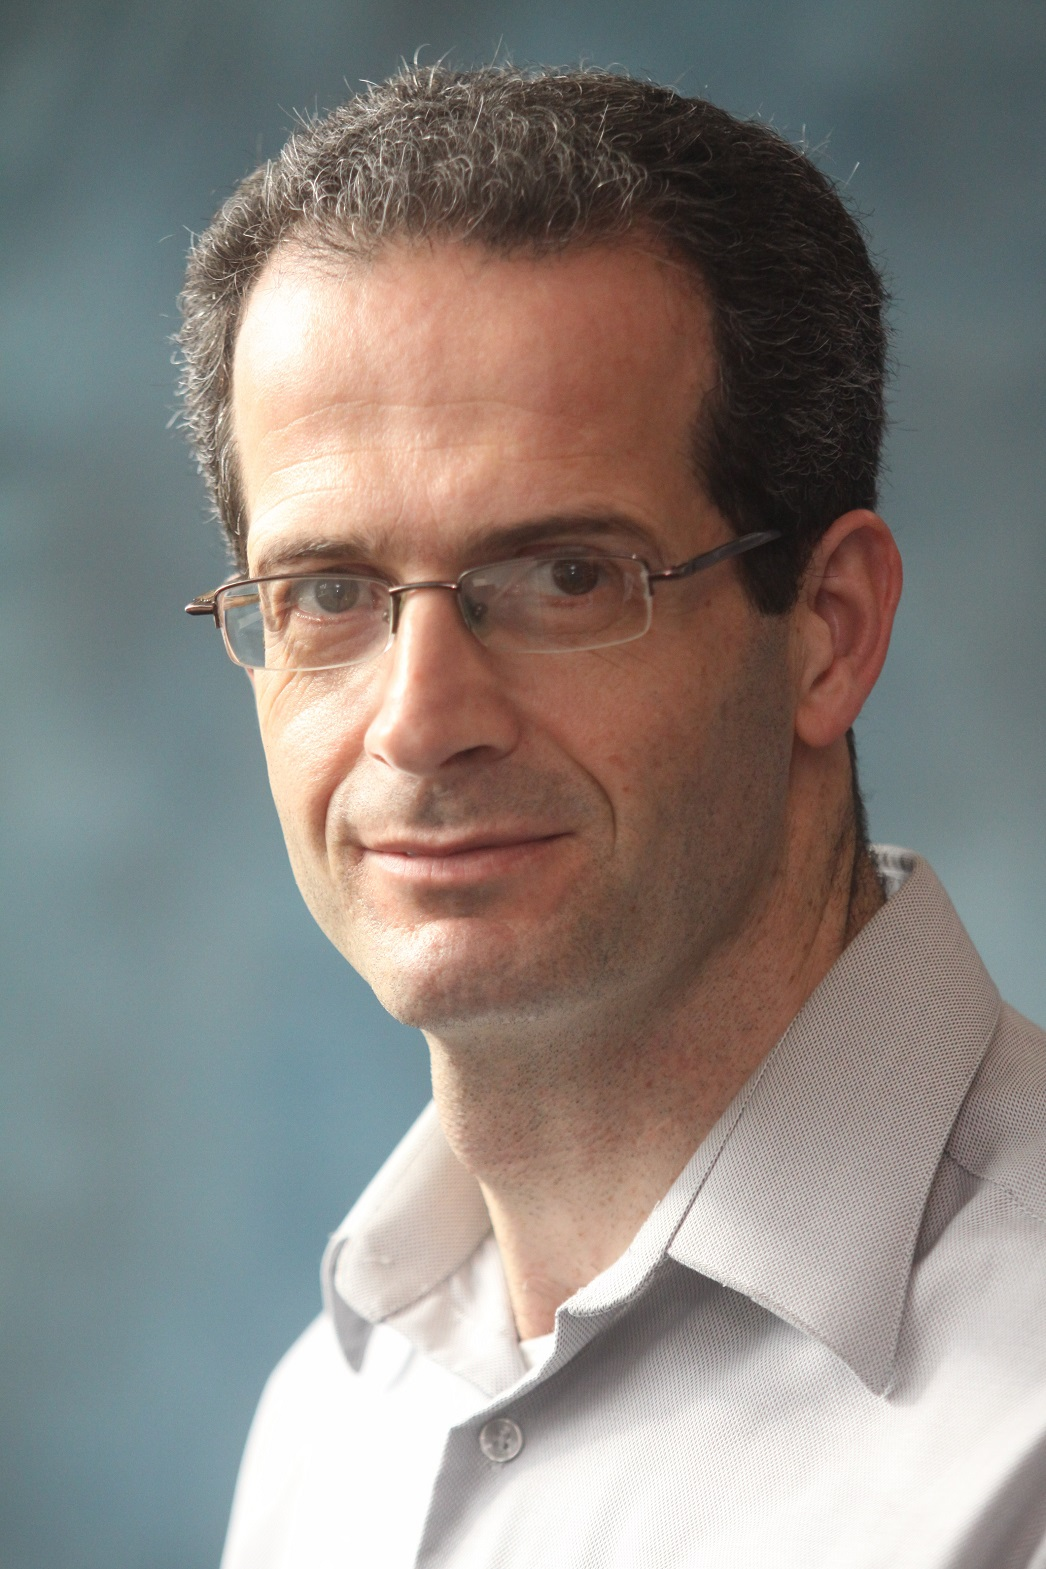
\includegraphics[width=1in,height
=1.25in,clip,keepaspectratio]{./Media/IsraelCohen.jpg}}]{Israel Cohen} (M'01-SM'03-F'15)
received the B.Sc. (Summa Cum Laude), M.Sc.
and Ph.D. degrees in electrical engineering from the Technion -- Israel Institute of
Technology, , Haifa, Israel, in 1990, 1993 and 1998, respectively.
He is currently the Louis and Samuel Seidan Professor in electrical engineering at the Technion -- Israel Institute of Technology.
He is also a Visiting Professor at Northwestern Polytechnical University, Xi’an, China.

From 1990 to 1998, he was a Research Scientist with RAFAEL Research
Laboratories, Haifa, Israel Ministry of Defense. From 1998 to 2001,
he was a Postdoctoral Research Associate with the Computer Science
Department, Yale University, New Haven, CT, USA. In 2001 he joined the
Electrical Engineering Department of the Technion.
%
He is a coeditor of the Multichannel Speech
Processing Section of the \textit{Springer Handbook of Speech
Processing} (Springer, 2008), and the coauthor of \textit{Fundamentals of Signal Enhancement and Array Signal Processing} (Wiley-IEEE Press, 2018).
%
His research interests are array processing, statistical signal processing, deep learning,
analysis and modeling of acoustic signals, speech enhancement, noise
estimation, microphone arrays, source localization, blind source
separation, system identification and adaptive filtering.

Dr. Cohen was the recipient of the Norman Seiden Prize for Academic Excellence (2017),
the SPS Signal Processing Letters Best Paper Award (2014),
the Alexander Goldberg Prize for Excellence in Research (2010),
and the Muriel and David Jacknow Award for Excellence in Teaching (2009).
He is an Associate Member of the IEEE Audio and Acoustic Signal Processing Technical Committee, and Distinguished Lecturer of the IEEE Signal Processing Society.
He was as Associate Editor of the \textsc{IEEE Transactions on Audio, Speech, and Language
Processing} and \textsc{IEEE Signal Processing Letters} and a Member of the IEEE Audio and Acoustic Signal Processing Technical Committee and the IEEE Speech and Language Processing Technical Committee.

\end{IEEEbiography}

\begin{IEEEbiography}[{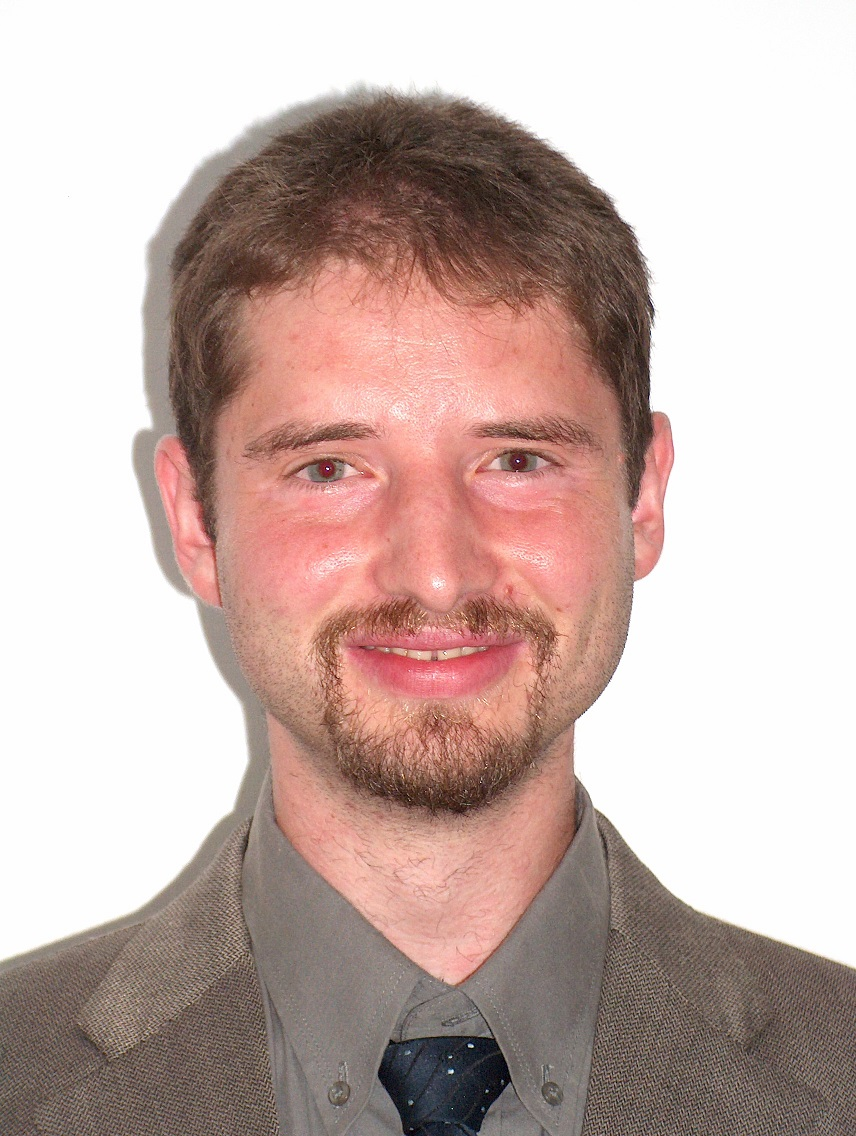
\includegraphics[width=1in,height=1.25in,clip,keepaspectratio]{./Media/dvorkind.JPG}}]{Tsvi G. Dvorkind}
received the B.Sc. degree (summa cum laude) in computer engineering in 2000, the M.Sc. degree (summa cum laude) in electrical engineering in 2003, and the Ph.D. degree in electrical engineering in 2007, all from the Technion—Israel Institute of Technology, Haifa, Israel.
From 1998 to 2000 he worked at the Electro-Optics Research & Development Company at the Technion, and during 2000–2001 at the Jigami Corporation.
He is now with the Rafael Company, Haifa, Israel.
His research interests include speech enhancement and acoustical localization, general parameter estimation problems, and sampling theory.
\end{IEEEbiography}
\begin{IEEEbiography}[{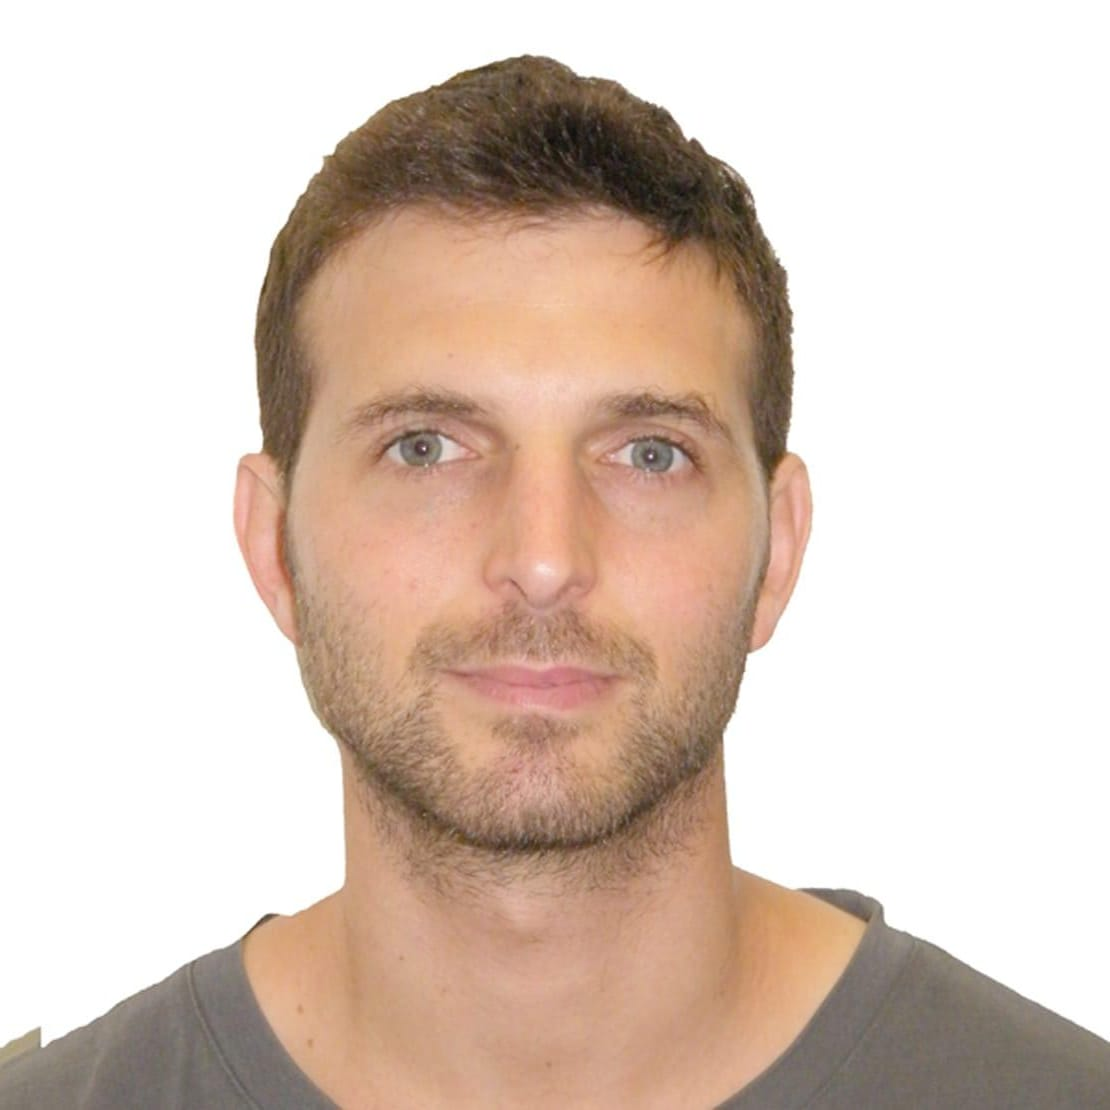
\includegraphics[width=1in,height=1.25in,clip,keepaspectratio]{./Media/Itay_Yehezkel_Karo.jpg}}]{Itay Yehezkel Karo}
received the B.Sc. degree in electrical engineering in 2013 from the Technion—Israel Institute of Technology, Haifa, Israel.
From 2010 to 2019 he worked at the Rafael Company, Haifa, Israel.
His research interest is mainly em signal-processing - especially array processing and spatial filtering.
\end{IEEEbiography}

% \begin{IEEEbiography}[{
\includegraphics[width=1in,height=1.25in,clip,keepaspectratio]{./Media/addPhotoHere.PNG}}]{Israel Cohen}
% (M’01–SM’03–F’15) He received the B.Sc. (Summa Cum Laude), M.Sc., and Ph.D. degrees in electrical engineering from the Technion – Israel Institute of Technology, Haifa, Israel, in 1990, 1993, and 1998, respectively.
% He is currently a Professor of electrical engineering with the Technion – Israel Institute of Technology.
% From 1990 to 1998, he was a Research Scientist with RAFAEL Research Laboratories, Israel Ministry of Defense, Haifa. 
% From 1998 to 2001, he was a Postdoctoral Research Associate with the Computer Science Department, Yale University, New Haven, CT, USA. In 2001, he joined the Electrical Engineering Department, Technion – Israel Institute of Technology.
% He is a coeditor of the Multichannel Speech Processing Section of the Springer Handbook of Speech Processing (Springer, 2008), and a coauthor of Fundamentals of Signal Enhancement and Array Signal Processing (Wiley-IEEE Press, 2017). 
% His research interests include array processing, statistical signal processing, analysis and modeling of acoustic signals, speech enhancement, noise estimation, microphone arrays, source localization, blind source separation, system identification, and adaptive filtering.
% Dr. Cohen was awarded the Norman Seiden Prize for Academic Excellence (2017), the SPS Signal Processing Letters Best Paper Award (2014), the Alexander Goldberg Prize for Excellence in Research (2010), and the Muriel and David Jacknow Award for Excellence in Teaching (2009). 
% He is currently an Associate Member of the IEEE Audio and Acoustic Signal Processing Technical Committee. 
% He was an Associate Editor for the IEEE TRANSACTIONS ON AUDIO, SPEECH, AND LANGUAGE PROCESSING and the IEEE SIGNAL PROCESSING LETTERS, and as Member of the IEEE Audio and Acoustic Signal Processing
% Technical Committee and the IEEE Speech and Language Processing Technical Committee.
% \end{IEEEbiography}
% \begin{IEEEbiography}[{
\includegraphics[width=1in,height=1.25in,clip,keepaspectratio]{./Media/addPhotoHere.PNG}}]{Tsvi G. Dvorkind}
% Tsvi G. Dvorkind received the B.Sc. degree (summa cum laude) in computer engineering in 2000, the M.Sc. degree (summa cum laude) in electrical engineering in 2003, and the Ph.D. degree in electrical engineering in 2007, all from the Technion—Israel Institute of Technology, Haifa, Israel.
% From 1998 to 2000 he worked at the Electro-Optics Research & Development Company at the Technion, and during 2000–2001 at the Jigami Corporation.
% He is now with the Rafael Company, Haifa, Israel.
% His research interests include speech enhancement and acoustical localization, general parameter estimation problems, and sampling theory.
% \end{IEEEbiography}
% \begin{IEEEbiography}{Itay Yehezkel Karo}
% Biography text here.
%\end{IEEEbiography}
\end{document}


